\section{Ordering and Asynchrony}
\label{sec:async}

% \begin{figure}[t]
%   \centering
%   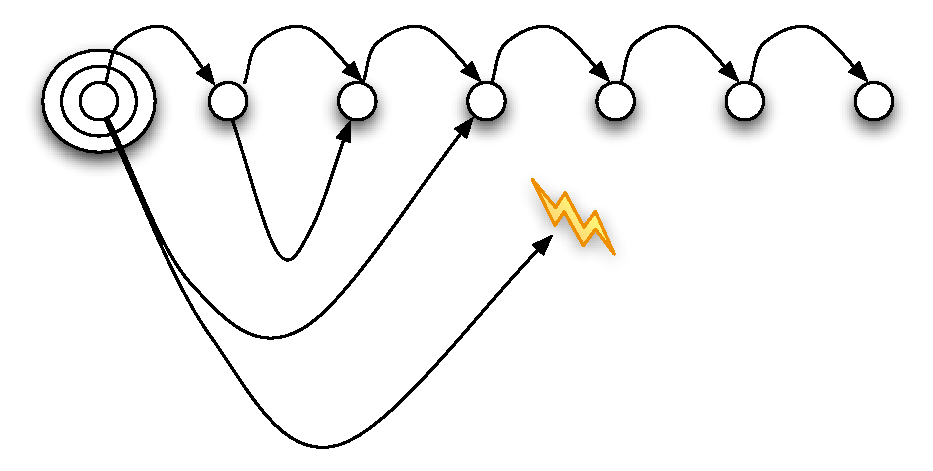
\includegraphics[width=0.75\linewidth]{figures/dedalus-time.pdf}
%   \label{fig:time}
%   %%\caption{Time moves forward in three ways: across strata, to the next fixpoint, and to some future fixpoint.}
%    \caption{Dedalus admits inferences whose consequences are visible immediately, in the next timestep, or at some unspecified timestep.}
%    
% \vspace{-8pt}
% \end{figure}

Until now we have restricted our discussion to \slang.  In this section we
introduce \lang, a superset of \slang that also admits the \emph{choice} construct~\cite{greedychoice} to bind time suffixes.
Choice allows us to model the inherent nondeterminism in communication over unreliable
networks that may delay, lose or reorder the results of logical deductions. 
We also describe a syntactic convention to employ this communication model for ``horizontal partitions'' of relations on different machines.
%(see Figure~\ref{fig:time}).

%%\subsection{{\bf \large \lang}: New Constructs}

\subsection{Choice}

%%In this section we present the Datalog extensions missing from \slang that we will need in \lang to capture important properties of practical distributed systems.  These include aggregate functions to 
%%capture ordering constraints, and---more importantly---the choice construct to capture nondeterminacy.


%%\subsubsection{Choice}
An important property of distributed systems is that individual computers cannot control or observe the temporal interleaving of their computations with other computers.  One aspect of this uncertainty is captured in network delays: the arrival ``time'' of messages cannot be directly controlled by either sender or receiver.  In this section, we enhance our language with a traditional model of nondeterminism from the literature to capture these issues: the \emph{choice} construct as defined by Greco and Zaniolo~\cite{greedychoice}.

The subgoal \dedalus{choose((\emph{$X_1$}), (\emph($X_2$))} may appear
in the body of a rule, where \emph{$X_1$} and \emph{$X_2$} are vectors
whose constituent variables occur elsewhere in the body.  Such a
subgoal enforces the functional dependency \emph{$X_1$} $\to$ $X_2$,
``choosing'' a single assignment of values to the variables in
\emph{$X_2$} for each variable in \emph{$X_1$}.

The choice construct is nondeterministic.  In a model-theoretic interpretation of logic programming, a nondeterministic program 
must have a multiplicity of stable models---that is it must be unstratifiable.  Greco and Zaniolo define 
choice in precisely this fashion: the choice construct is expanded into an unstratifiable strongly-connected component of rules, 
and each possible choice is associated with a different model.  Each such model has a unique, non-deterministic assignment that
respects the given functional dependencies.  In our discussion, it may be helpful to think of one such model chosen non-deterministically---a non-deterministic ``assignment of timestamps to tuples''.

%%\paa{significantly, for any choice, the resulting program has a unique minimal model if the program (independent of the choice expansion)
%%is stratifiable, locally stratifiable, etc}  \jmh{You do need to resolve the previous paragraph, or rewrite it to simply say ``see the Italians if you want to understand more, 
%%but for our purposes assume a unique non-deterministic assignment that respects the FDs.  This allows us to have agreed-upon minimal models.''}

\subsection{Distribution Model}
The choice construct will capture the non-determinism of multiple communicating agents in a distributed system, but we want to use it in a stylized way to model typical notions of distribution.  To this end \lang adopts the ``horizontal partitioning'' convention introduced by Loo, et al.\ and used in many subsequent efforts~\cite{Loo:2005}.
To represent a distributed system, we consider some number of agents,
each running a copy of the same program against a disjoint subset ({\em
  horizontal partition}) of each predicate's contents.  We require one
attribute in each predicate to be used to identify the
partitionining for tuples in that predicate. We call such an
attribute a {\em location specifier}, and prefix it with a
\dedalus{\#} symbol in Dedalus.

Finally, we constrain \lang rules so that the location specifier variable in each body predicate be the same---i.e. the body contains tuples from exactly one partition of the database, logically colocated (on a single ``machine'').  If the head of the rule has the same location specifier variable as the body, we call the rule ``local'', since its results can remain on the machine where they are computed.  If the head has a different variable in its location specifier, we call the rule a {\em communication rule}.  We now proceed to our model of the asynchrony of this communication, which is captured in a syntactic constraint on the heads of communication rules.

\subsection{Asynchronous Rules}

In order to represent the nondeterminism introduced by distribution, we admit a
third type of rule, called an {\em asynchronous} rule.  A rule is asynchronous
if the 
%Recall our use of the distinguished variables $\Tau$ and $S$ to represent the
%time suffixes respectively in the body and head of a rule
%(Section~\ref{sec:syntaxrestrictions}).  in our discussion of \slang,
%representing the time suffixes occuring respectively in the body and head of a
%rule.
relationship between the head time suffix $\SDedalus$ and the body time suffix $\Tau$ is
unknown.  Furthermore, $\SDedalus$ (but not $\Tau$) may take on the special value
$\top$ which means ``never.''  Derivation at $\top$ indicates that the
deduction is ``lost,'' as time suffixes in rule bodies do not range over
$\top$.

We model network nondeterminism using the choice construct to choose
from a value in the special 
%%\dedalus{successors} 
\dedalus{time}
predicate, which is defined using the following Datalog rules:

\begin{Dedalus}
time(\(\top\));
time(\(\SDedalus\)) \(\leftarrow\) successor(\(\SDedalus\), _);
\end{Dedalus}

\noindent
Each asynchronous rule with head predicate \dedalus{p($A_1, \ldots, A_n$)} has the following additional subgoals in its
body:

\dedalus{time($\SDedalus$), choose(($A_1, \ldots, A_n, \Tau$), ($\SDedalus$))}, 

\noindent
where
$\SDedalus$ is the timestamp of the rule head.  Note that our use of \dedalus{choose} incorporates all variables of each head predicate tuple, which allows a unique choice of $\SDedalus$ for each head tuple.


\begin{example}
A well-formed asynchronous \lang rule:

\begin{Dedalus}
r(A, B, \(\SDedalus\)) \(\leftarrow\) 
  e(A, B, \(\Tau\)),
  time(\(\SDedalus\)), choose((A, B, \(\Tau\))), (\(\SDedalus\)));
\end{Dedalus}
\end{example}

We admit a new temporal head annotation to sugar the rule above.  The
identifier \dedalus{async} implies that the rule is asynchronous, and stands in for
the additional body predicates.
%%$N$ is a variable,
%%corresponding to the time suffix $\Tau$ of all predicates in the rule body and
%%optionally referenced in the head.  
The above example expressed using \dedalus{async} is:

% asynchronous
\begin{example}
	A sugared asynchronous \lang rule:
	
\begin{Dedalus}
r(A, B)@async \(\leftarrow\) e(A, B);
\end{Dedalus}
\end{example}

\subsection{Asynchrony and Distribution in {\large{\bf\lang}}}
As a syntactic constraint of \lang, the {\em communication rules} introduced in the previous section (rules that differ in head and body location specifiers) are required to be asynchronous.
This restricts our model of communication between agents in two important ways.
First, by restricting bodies to a single agent, the only communication
modeled in \lang occurs via communication rules.  Second, because
all communication rules are asynchronous, agents may only learn about
time values at another agent by receiving messages (with unbounded
delay) from that agent.  Note that this model says nothing about the
relationship between the agents' clocks; they could be
non-monotonically increasing, or they could respect a global order.

\subsection{Temporal Monotonicity}


Nothing in our definition of asynchronous rules prevents tuples in the
head of a rule from having a timestamp that precedes the timestamp in
the rule's body. This is a significant departure from \slang, since it
violates the monotonicity assumptions upon which we based both Algorithm~\ref{alg:tsn} and our proof of
temporal stratification.  On an intuitive level, it may also trouble
us that rules can derive head tuples that exist ``before'' the body
tuples on which they are grounded; this violates intuitive notions of
causality and admits the possibility of temporal paradoxes.

We have avoided restricting \lang to rule out such issues, as doing so
would reduce its expressiveness.  Recall that simple monotonic Datalog (without negation) is insensitive to the values in any particular attribute.  Hence \lang programs without negation are also well-defined regardless of any ``temporal ordering'' of deductions: in monotonic programs, even if tuples with timestamps ``in the future'' are used to derive tuples ``from the past'', there is an unambiguous least minimal model.

For non-monotonic \slang programs, the monotonicity of the time suffix ensures us a unique minimal model in many cases.  Whenever we can guarantee monotonicity of the time suffix for \lang programs, our results from Section~\ref{sec:strat} still apply for all models produced by the choice construct.

% Recall, however, that
% Algorithm~\ref{alg:tsn} assumed some sort of temporal monotonicity
% property, which we will now define.

%
%and that with monotonicity of time, we get
%\rcs{foo}, monotonicity of rules we get \rcs{bar}, and with
%monotonicity of neither, we get unstratifiable Datalog
%programs. \rcs{everything after recall is up in the air...}

% If we assume that our executions obey some causal ordering, then we
% know there is some partial order over the rule derivations of the
% system, and therefore, there exists at least one total ordering of the
% execution that corresponds to the partial order.  Therefore, each
% execution of a \lang program (which may be nondeterministic due to
% \dedalus{@async}) is equivalent to the execution of some deterministic \slang
% program; these causality assumptions reintroduce the temporal stratifiability
% that our definition of \lang gave up.
% 
% Similarly, if we disallow negation, but allow derivations to travel
% backwards in time, the resulting \lang program is still temporally
% stratifiable.  However, admitting both negation across timesteps and
% causality violations leads to an underlying Datalog program that is
% unstratifiable.
\subsubsection{Practical Implications}
Given this discussion, in practice we are interested in three asynchronous scenarios: (a) monotonic programs (even with non-monotonicity in time), (b) non-monotonic programs whose semantics guarantee monotonicity of time suffixes  and (c) non-monotonic programs where we have domain knowledge guaranteeing monotonicity of time suffixes.  Each represents practical scenarios of interest.

The first category captures the spirit of many simple distributed implementations that are built atop unreliable asynchronous substrates.  For example, in some Internet publishing applications (weblogs, online fora), it is possible due to caching or failure that a ``thread'' of discussion arrives out of order, with responses appearing before the comments they reference.  In many cases a monotonic ``bag semantics'' for the comment program is considered a reasonable interface for readers, and the ability to tolerate temporal anomalies simplifies the challenge of scaling a system through distrbution.

The second scenario is achieved in \slang via the use of \dedalus{successor} for the time suffix. The asynchronous rules of \lang require additional program logic to guarantee monotonic increases in time for predicates with dependencies.  In the theoretical literature of distributed computing, this is known as a {\em causal ordering}, and is enforced by distributed clock protocols.  We review one classic protocol in the \lang context in Section~\ref{sec:lamport}; including this protocol into \lang programs ensures temporal monotonicity.

Finally, certain computational substrates guarantee monotonicity in both timestamps and message ordering -- for example, som multiprocessor cache coherency protocols achieve this.  When temporal monotonicity is given, the proofs of temporal stratification and Algorithm~\cite{alg:tsn} both apply.

\subsubsection{Entanglement}
\label{sec:entangle}
Consider the asynchronous rule below:

\begin{Dedalus}
p(A, B, N)@async \(\leftarrow\)
  q(A, B)@N;
\end{Dedalus}
\noindent
Due to the \dedalus{async} keyword in the rule head, each \emph{p} tuple will take some unspecified time suffix value.
Note however that the time suffix $N$ of the rule body appears also in an attribute of \emph{p} other than the time suffix, recording a 
binding of both the time value of the deduction and the time value of its consequence.  We call such a binding
an \emph{entanglement}.   Note that in order
to write the rule it was necessary to not sugar away the time suffix in the rule body.  

Entanglement is a powerful construct.  It allows a rule
to reference the logical clock time of the deduction that produced one
(or more) of its subgoals; this supports protocols that reason about partial ordering of time across machines.  More generally, it exposes the infinite \dedalus{successor} relation to attributes other than the time suffix, allowing us to express concepts such as infinite sequences.

%%\jmh{Where do we give the def that say ``\lang is \slang with the following extra goo''?  Here?  After async?}\rcs{beginning of sec 6, first sentence}

\subsection{Lamport Clocks}
\label{sec:lamport}
Recall that \lang allows program executions to order message timestamps arbitrarily, violating intuitive notions of causality by allowing deductions to ``affect the past''.
This section explains how to implement Lamport
clocks~\cite{timeclocks} atop \lang, which allows programs to ensure
temporal monotonicity, by reestablishing a causal order
despite derivations that flow backwards through time.

Consider a rule \dedalus{p(A,B)@async \(\leftarrow\) q(A,B)}.  By
rewriting it to:

\begin{Dedalus}
persist[p, p\_neg, 2]
p\_wait(A, B, N)@async \(\leftarrow\) q(A, B)@N;
p\_wait(A, B, N)@next \(\leftarrow\) p\_wait(A, B, N)@M, N \(\ge\) M;
p(A, B)@next \(\leftarrow\) p\_wait(A, B, N)@M, N < M;
\end{Dedalus}
\noindent
we place the derived tuple in a new relation \dedalus{p\_wait} that
stores any tuples that were ``sent from the future'' with their sending time ``entangled''; these tuples stay in the \dedalus{p\_wait} predicate  until the point in
time at which they were derived.  Conceptually, this causes the system
to evaluate a potentially large number of timesteps (if N is
significantly less than the timestamp of the system when the tuple
arrives).  However, if the runtime is able to efficiently evaluate
timesteps when the database is quiescent, then
instead of ``waiting'' by evaluating timesteps, it will simply
increase its logical clock to match that of the sender.  In contrast,
if the tuple is ``sent into the future,'' then it is processed using
the timestep that receives it.

This manipulation of timesteps and clock values is equivalent to
conventional descriptions of Lamport clocks, except that our Lamport
clock implementation effectively ``advances the clock'' by preventing derivations until the clock is sufficiently advanced, by temporarily store incoming tuples
in the \dedalus{p\_wait} relation.

We gloss over one detail here: Lamport clocks rely
upon a ``tie-breaking'' function to ensure that no two events have the
same timestamp.  In \lang, such a function could be implemented via another use of \dedalus{choice}, or by a program convention like
appending a unique node identifier to each timestamp to prevent ``ties''.

%%\jmh{Can't we please do the normal use of Lamport clocks, i.e. show how it solves a distributed systems problem?}
%%\rcs{I'd like to do this, but don't have any good examples...}
